\documentclass[12pt]{article}
\usepackage[utf8]{inputenc}
\usepackage{geometry}
\usepackage{amsmath, amssymb}
\usepackage{graphicx}
\usepackage{hyperref}
\geometry{a4paper, margin=1in}
\usepackage{transparent}
\usepackage{amsfonts}
\usepackage{listings}
\usepackage{xcolor}
\usepackage{float}
\usepackage{transparent}

\title{Proyecto 3}

\date{}

\begin{document}

\maketitle

\begin{center}
    \textbf{Matemática Discreta sección 30}
\end{center}

\begin{figure}[H]
    \centering
    \transparent{0.5}
    
\includegraphics[width=0.55\linewidth]{Logo.png}
    \label{fig:placeholder}
\end{figure}

\begin{center}
    Paula de León \\
    Isaías García \\
    Natanael Girón \\
    Jimberth Maldonado \\
    Pablo Méndez \\
    Karen Pineda
\end{center}

\begin{center}
    Ciudad de Guatemala, Guatemala \\
    Octubre de 2025
    
\end{center}

\newpage

\tableofcontents
\newpage

\section{Introducción}
El documento corresponde al proyecto 3 del curso \textbf{Matemática Discreta 1 (MM2015)} de la Universidad del Valle de Guatemala. 
El objetivo principal es implementar, mediante un programa en Python, las diferentes técnicas de conteo fundamentales, específicamente 
\textbf{permutaciones y combinaciones}, tanto para objetos diferentes como para objetos iguales.

El programa desarrollado en consola permite que el usuario defina conjuntos, cree relaciones y calcule automáticamente
todas las combinaciones y permutaciones posibles. Los resultados se muestran paso a paso y se explican con las fórmulas 
utilizadas, lo que facilita la comprensión del tema.

\section{Estructura del Programa}
El programa está diseñado de forma modular e interactiva, integrando los temas previos de conjuntos y relaciones
con las nuevas funcionalidades de conteo. Desde el menú principal, el usuario puede acceder a las siguientes opciones:

\begin{enumerate}
    \item Definir conjunto referencial (universo)
    \item Crear nuevos conjuntos o relaciones
    \item Ejecutar operaciones de conjuntos (unión, intersección, diferencia, complemento)
    \item Calcular producto cartesiano
    \item Verificar propiedades de relaciones (reflexiva, simétrica, transitiva)
    \item Calcular permutaciones y combinaciones:
    \begin{itemize}
        \item Permutaciones de objetos diferentes
        \item Permutaciones de objetos iguales
        \item Combinaciones de objetos diferentes
        \item Combinaciones de objetos iguales
    \end{itemize}
\end{enumerate}

\section{Fundamento Teórico: Técnicas de Conteo}
\subsection{Permutaciones}
El programa implementa dos tipos principales de permutaciones:

\begin{itemize}
    \item \textbf{Permutaciones de objetos diferentes:}
    \[
        P(n,r) = \frac{n!}{(n-r)!}
    \]
    Donde $n$ es el número total de elementos y $r$ el número de elementos a permutar.
    
    \item \textbf{Permutaciones de objetos iguales:}
    \[
        P(n; n_1, n_2, ..., n_k) = \frac{n!}{n_1!n_2!...n_k!}
    \]
    Esta fórmula se utiliza cuando existen elementos repetidos dentro del conjunto.
\end{itemize}

\subsection{Combinaciones}
Se implementaron dos tipos de combinaciones:

\begin{itemize}
    \item \textbf{Combinaciones de objetos diferentes (sin repetición):}
    \[
        C(n,r) = \binom{n}{r} = \frac{n!}{r!(n-r)!}
    \]
    
    \item \textbf{Combinaciones de objetos iguales (con repetición):}
    \[
        C_R(n,r) = \binom{n+r-1}{r} = \frac{(n+r-1)!}{r!(n-1)!}
    \]
\end{itemize}

\section{Descripción de la Implementación}
\subsection{Gestión de Conjuntos y Relaciones}
El código utiliza clases en Python para mantener una estructura organizada.  
El objeto principal \texttt{RelacionesApp} permite:
\begin{itemize}
    \item Crear y modificar conjuntos
    \item Definir un universo referencial
    \item Crear relaciones entre conjuntos
    \item Ejecutar operaciones lógicas sobre conjuntos
\end{itemize}

\subsection{Funciones de Conteo}
Los métodos \texttt{combinaciones\_objetos\_diferentes}, 
\texttt{combinaciones\_objetos\_iguales}, 
\texttt{permutaciones\_objetos\_diferentes} y 
\texttt{permutaciones\_objetos\_iguales} implementan las fórmulas descritas usando el módulo \texttt{itertools} y las funciones \texttt{factorial()} y \texttt{Counter()} de Python.

Cada cálculo imprime:
\begin{itemize}
    \item Todas las combinaciones o permutaciones generadas
    \item La fórmula aplicada
    \item El total de resultados obtenidos
\end{itemize}

\subsection{Interfaz Interactiva}
El programa ejecuta un menú en consola con 18 opciones numeradas.  
El usuario ingresa el conjunto, el valor de $k$ (cuando aplica) y elige si desea realizar una combinación o permutación, con o sin repetición.

\section{Resultados y Ejemplos}

\subsection{Ejemplo 1: Permutaciones de Objetos Diferentes}

\begin{figure}[H]
    \centering
    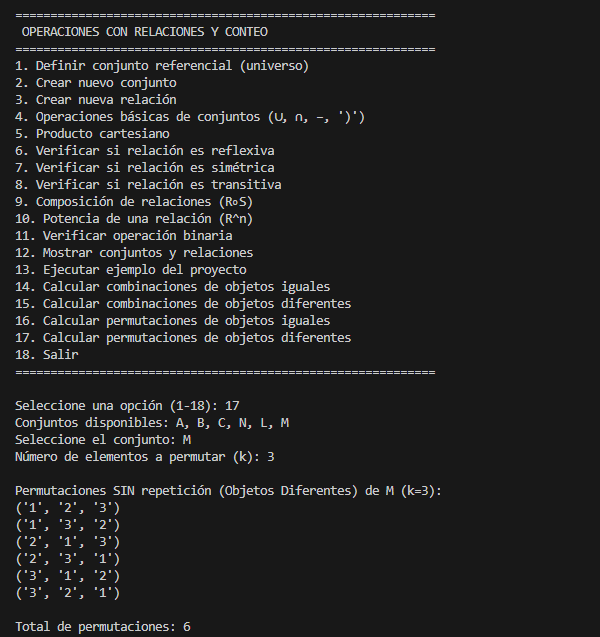
\includegraphics[width=0.85\textwidth]{Foto1.png}
    \caption{Ejecución en consola - Permutaciones de objetos diferentes}
\end{figure}

\subsection{Ejemplo 2: Permutaciones de Objetos Iguales}

\begin{figure}[H]
    \centering
    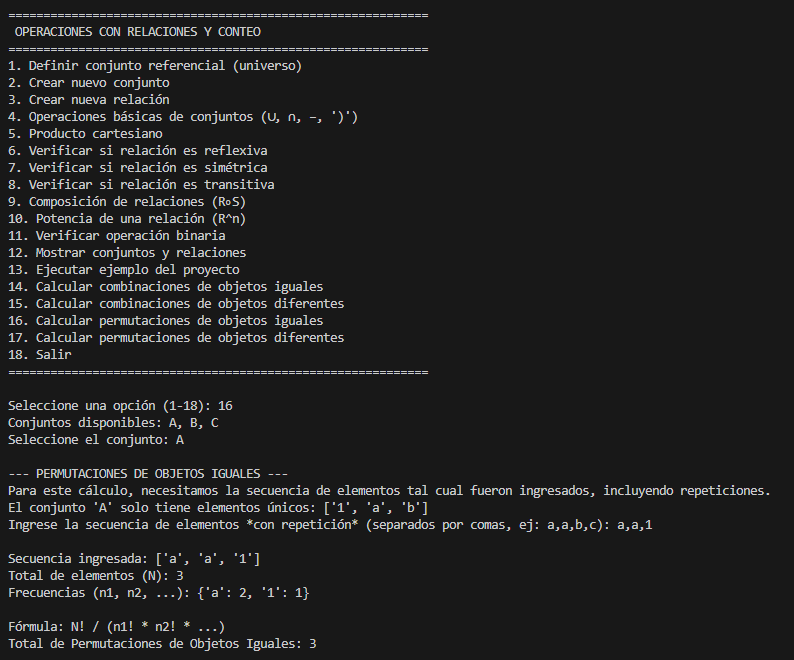
\includegraphics[width=0.85\textwidth]{Foto2.png}
    \caption{Ejecución en consola - Permutaciones de objetos iguales}
\end{figure}

\subsection{Ejemplo 3: Combinaciones de Objetos Diferentes}

\begin{figure}[H]
    \centering
    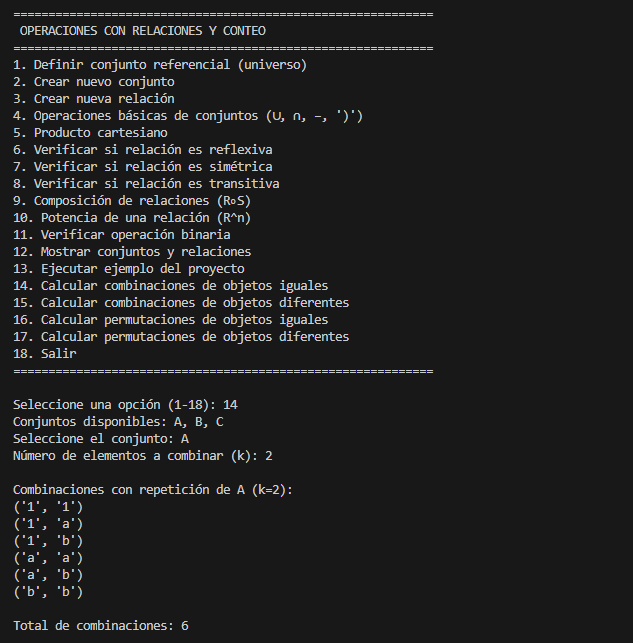
\includegraphics[width=0.85\textwidth]{Foto3.png}
    \caption{Ejecución en consola - Combinaciones de objetos diferentes}
\end{figure}

\subsection{Ejemplo 4: Combinaciones de Objetos Iguales}

\begin{figure}[H]
    \centering
    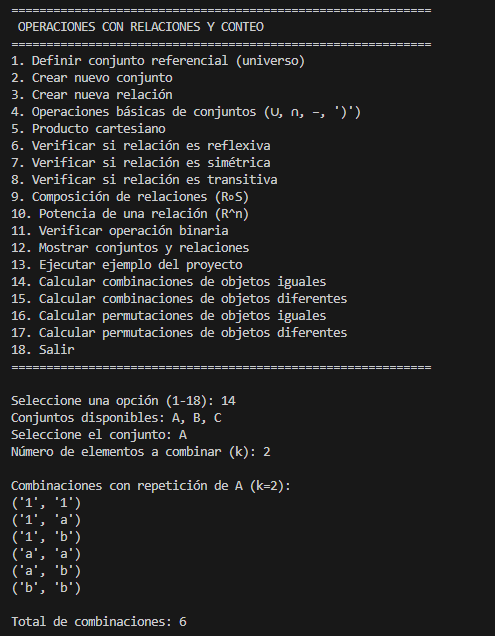
\includegraphics[width=0.85\textwidth]{Foto4.png}
    \caption{Ejecución en consola - Combinaciones de objetos iguales}
\end{figure}

\section{Detalles Técnicos}
\begin{itemize}
    \item Lenguaje utilizado: Python 3
    \item Librerías: \texttt{itertools}, \texttt{math}, \texttt{collections}, \texttt{re}
    \item Entrada y salida: consola interactiva
    \item Validación: manejo de errores, vacíos y casos extremos
    \item Total de opciones en menú: 18
\end{itemize}

\section{Conclusiones}
\begin{enumerate}
    \item La implementación en Python permitió aplicar los conceptos de permutaciones y combinaciones de forma práctica e interactiva.
    \item El programa integra tanto objetos diferentes como iguales, abarcando todos los tipos de conteo vistos en clase.
    \item Las fórmulas se validan con resultados generados por código, fortaleciendo la comprensión teórica.
    \item La estructura modular del código facilita su extensión para incluir nuevos temas de Matemática Discreta.
    \item Se resolvieron problemas de indentación y definición de métodos, asegurando la ejecución sin errores.
\end{enumerate}

\section{Referencias}
\begin{itemize}
    \item Rosen, K. (2019). \textit{Discrete Mathematics and Its Applications} (8th ed.). McGraw-Hill.
    \item Universidad del Valle de Guatemala. (2025). \textit{Matemática Discreta 1 (MM2015)}.
\end{itemize}

\end{document}